\documentclass{article}

\usepackage{amsmath}
\usepackage{amssymb}
\usepackage{amsxtra}
\usepackage{graphicx}
\usepackage{listings}
\usepackage{subcaption}
\usepackage{wrapfig}
\usepackage{todonotes}
\usepackage{url}
\usepackage[margin=1.2in]{geometry}

\newcommand{\refchapter}[1]{Chapter~\ref{#1}}
\newcommand{\refsec}[1]{Section~\ref{#1}}
\newcommand{\refeqn}[1]{Equation~(\ref{#1})}
\newcommand{\reffig}[1]{Figure~\ref{#1}}

\title{\bf Software Lab \\ Computational Engineering Science \\
{\Large Pusher Mechanism}} 

\vspace{1.5cm}

\author{Aaron Albert Floerke, Arseniy Kholod, Xinyang Song, Yanliang Zhu \\[1cm]Supervisor: Dr. rer. nat. Markus Towara\footnote{Informatik 12: Software and Tools for Computational Engineering, RWTH Aachen University, {\tt info@stce.rwth-aachen.de}}}


\date{{\begin{center} 18\textsuperscript{th} November 2024 \end{center}} 
\includegraphics[width=.6\textwidth]{rwth_i12_softw-werkz_en_rgb}}

\begin{document}

\lstloadlanguages{Python}
\lstset{basicstyle=\small, numbers=left, numberstyle=\footnotesize,
  stepnumber=1, numbersep=5pt, breaklines=true, escapeinside={/*@}{@*/}}

\pagestyle{plain}

\maketitle

\clearpage

\section*{Preface}

The topic "Pusher Mechanism" was assigned as a final project by the Department of Informatik 12: Software and Tools for Computational Engineering, RWTH Aachen University, for the Software Lab course in the Computational Engineering Science B.Sc. program. This work was carried out under the supervision of Dr. rer. nat. Markus Towara.

This project involves developing an enhanced version of the well-known planar four-bar linkage, a mechanical system widely used in applications like conveyor systems, oil well pumps, and robotic arms. By adding an extra joint, the extended mechanism offers more degrees of freedom, making it better suited for specific tasks. In this work, we designed and implemented this extended four-bar linkage to find a suitable mechanism for moving a box along a conveyor while avoiding obstacles.

In the first phase of the project, we analyzed the user requirements provided by our supervisor and broke them down into system requirements. This was followed by a theoretical analysis of the mechanism's geometry. Based on this analysis, we selected Python as the implementation environment due to its suitability for the task and the team's expertise.

The implementation consists of three interconnected components. First, the backend was developed to handle the geometry of the linkage, calculating the coordinates of all joints based on input parameters to ensure accurate modeling.

The second component is the frontend, a graphical user interface (GUI) created with the Tkinter\footnote{https://docs.python.org/3/library/tkinter.html} library. It enables users to visualize the linkage’s movement, modify its parameters, and display essential information about the mechanism.

Additionally, a well-documented testing process was carried out to ensure the correctness and reliability of both the backend and frontend. This testing verified the system's performance across various scenarios, ensuring its accuracy and robustness.

With our implementation, we successfully addressed the optimization problem of moving a box along a conveyor while avoiding obstacles. The addition of an extra joint to the four-bar linkage provided the necessary degrees of freedom, enabling precise trajectory design. This solution met the system and user requirements and demonstrated the mechanism's effectiveness in achieving task-specific motion.

Furthermore, detailed documentation of the software and project management processes was created to enhance maintainability and offer a clear understanding of the project’s structure. This documentation ensures that future developers or users can efficiently modify and extend the system. Overall, this work demonstrates the successful combination of theoretical analysis, design, and practical implementation in creating a functional pusher mechanism.

\clearpage

\section{Introduction}

The industrial revolution in the 18th and 19th centuries brought about significant advancements in manufacturing processes, one of which was the challenge of transporting products efficiently between various workstations in factories. A key solution to this challenge was the development of mechanical systems like the four-bar linkage, which can be used as a pusher mechanism to move products along production lines or between different conveyor systems. Despite its simple structure, the four-bar linkage has proven to be an effective mechanism in various industrial applications. 

Over time, the four-bar linkage model has expanded beyond basic conveyor systems and has found applications in more complex systems, such as pumpjacks, robotic arms, and automotive engineering. Its simplicity and efficiency continue to make it relevant in modern mechanical design.

In this work, we aim to analyze the theoretical principles behind the four-bar linkage, design and implement an extended version of the mechanism with an additional joint, named coupler (see Figures \ref{fig:linkage-1} and \ref{fig:linkage-2}), and apply it to solve the problem of moving a box along a production line while avoiding obstacles. By enhancing the classic four-bar linkage, we seek to provide a more flexible solution suited to complex real-world tasks.

\begin{figure}[h]
	\centering
	\begin{subfigure}{0.49\textwidth}
		\centering
	    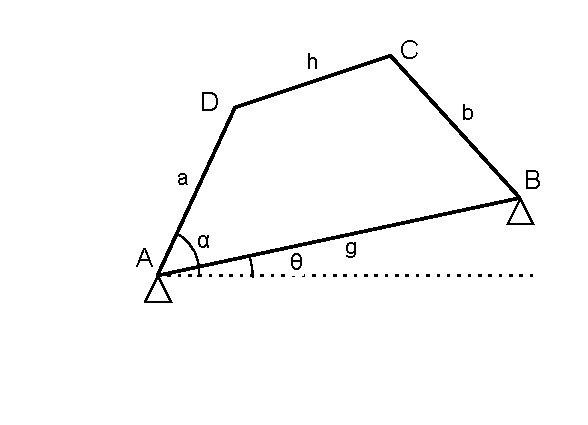
\includegraphics[width=\linewidth]{./figures/four-bar_linkage.pdf}
	    \caption{Planar four-bar linkage}
	    \label{fig:linkage-1}
	\end{subfigure}
	\hfill
	\begin{subfigure}{0.49\textwidth}
		\centering
		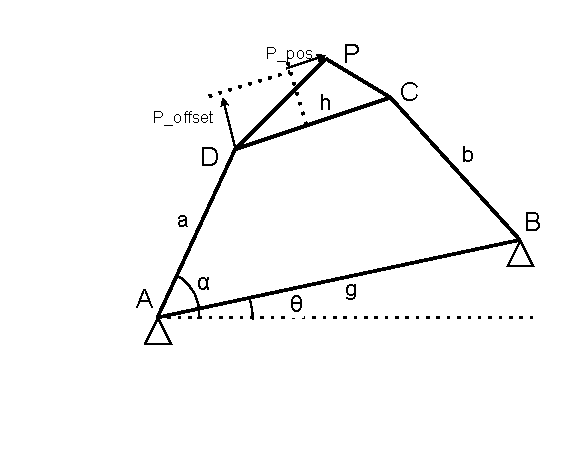
\includegraphics[width=\linewidth]{./figures/four-bar_linkage+coupler.pdf}
		\caption{Planar four-bar linkage with coupler $P$}
		\label{fig:linkage-2}
	\end{subfigure}
	\caption{Four-bar linkage}
\end{figure}

The structure of this paper is as follows: In Section \ref{ch:analysis}, we analyze the user requirements, derive the system requirements, and provide an overview of the theoretical analysis of the mechanism’s geometry. Section \ref{ch:design} covers the selection of the implementation environment, taking into account the system requirements and the team's expertise, as well as the preparation of UML class models for the implementation phase. Section \ref{ch:implementation} describes the implementation of the four-bar linkage, the graphical user interface, and the software testing process, while Section \ref{ch:doc} provides software documentation to ensure its maintainability. In Section \ref{ch:optimization-problem}, we use the developed software to determine the appropriate mechanism parameters to move the box along the conveyor. Finally, in Sections \ref{ch:projectmanagement}, we discuss our project management.

\section{Analysis} \label{ch:analysis}

\subsection{User Requirements}

\begin{figure}[h]
	\centering
	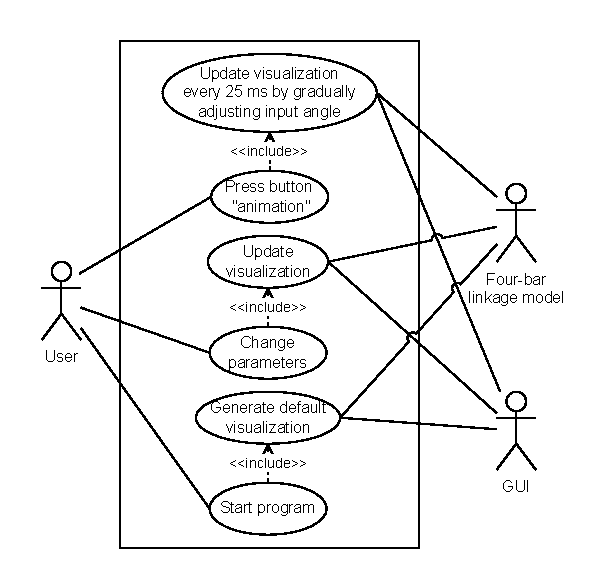
\includegraphics[width=0.7\textwidth]{./figures/uml_use_case.pdf}
	\caption{UML use case diagram}
	\label{fig:use_case}
\end{figure}

User requirements outline the overall vision for how a system should function and what features it must provide to meet user needs. These high-level expectations are the foundation for developers to derive more detailed and technical system requirements, which define constraints and specifications the software must fulfill.

To enhance understanding of the user requirements described later, we provide a UML use case diagram of user-software interactions in Figure \ref{fig:use_case}. The diagram illustrates the main workflow: after starting the program, the user is presented with a default visualization of the four-bar linkage generated by the GUI and the linkage model. The user can modify this visualization by specifying input parameters through the GUI. Additionally, the four-bar linkage can be animated, with the input angle gradually increasing and the visualization updating every 25 ms upon the user’s explicit request.

The following list presents all the user requirements provided by our supervisor, along with our explanations and interpretations of each concept.

\begin{itemize}
	\item \textit{Requirement: Implement all motion types of a planar four-bar linkage extended with a coupler.}
	
	The planar four-bar linkage extended with a coupler, illustrated in Figure \ref{fig:linkage-2}, may appear to be a straightforward geometric structure. However, its motion is more complex than it seems. While the coupler $P$ does not influence the primary motion constraints, the lengths of the four main bars define the limitations of the input angle $\alpha$. These constraints can result in the input angle being unlimited, symmetrically limited, or asymmetrically limited relative to the ground link $AB$. Consequently, the links $AD$ and $BC$ can function as either cranks, capable of full rotation, or rockers, which only partially rotate. In fact, as explained in \cite{inproceedings}, 27 distinct motion types for such mechanisms have been identified. A deeper analysis of these motion types will be conducted in the theoretical section of our study.
	
	\item \textit{Requirement: Implement a graphical user interface (GUI) to display four-bar linkage animation and customize its geometric parameters.}
	
	The GUI should enable users to visualize the linkage, provide smooth animations, and adjust various geometric parameters of the system. We have identified eight key parameters (degrees of freedom, shown in Figure \ref{fig:linkage-2}) that the GUI should support:
	\begin{itemize}
		\item The lengths of the four bars ($AB$, $BC$, $CD$, $AD$).
		\item The angle $\theta$ between the fixed bar $AB$ and the horizontal line.
		\item The input angle $\alpha$ between the bar $AD$ and the horizontal line.
		\item The position of the coupler relative to the middle of the floating link, expressed by $P_{pos}$ and $P_{offset}$.
	\end{itemize}
	During the animation process, the input angle $\alpha$ is no longer a free parameter, as it is dynamically determined by the system to ensure smooth motion.
	
	Additionally, while the position of point $A$ could be considered an independent parameter (technically two parameters in 2D), for simplicity, we assume it is fixed at $(0, 0)$ during geometric analysis. If point $A$ needs to be positioned elsewhere, the entire linkage can simply be translated accordingly. This fixed-point assumption will simplify the design phase but can be revisited for solving optimization problems later.
	
	\item \textit{Requirement: Determine suitable parameters for the four-bar linkage to solve the following optimization problem:}
	\begin{itemize}
		\item Push box with size $80\times60$ from $x=220$ to $x=0$
		\item Do not cross the area of the labeling machine (Area with $x<80$ and $y>70$).
		\item Pass above points $(120, 80)$ and $(220, 80)$
	\end{itemize}
	
	\begin{figure}[h]
		\centering
		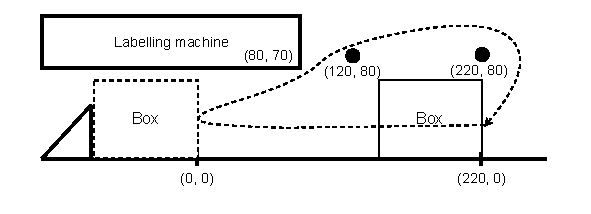
\includegraphics[width=0.7\textwidth]{./figures/optimization_problem_task.pdf}
		\caption{Optimization problem}
		\label{fig:optimization_problem}
	\end{figure}
	
	The optimization problem is illustrated in Figure  \ref{fig:optimization_problem}, which shows a conveyor line with the box to be moved by the coupler $P$ while avoiding the forbidden areas. The coupler $P$ must move the box, following a trajectory such as the dotted curve depicted in the figure. After pushing the box to the desired location, the coupler should return to its starting position, navigating around obstacles to repeat the task.
	
	At a minimum, the problem can be addressed manually by experimenting with different parameters to find a feasible solution. Ideally, however, an algorithm could be developed to automate the optimization process and identify the best parameters efficiently.
\end{itemize}

\subsection{System Requirements}

After reviewing and analyzing the user requirements, which provide a high-level perspective of the problem and its solution, we need to derive more detailed technical requirements and specifications for the software. The system requirements are categorized into two types: \textit{functional requirements}, which define what the software must do, and \textit{non-functional requirements}, which outline how the system should operate and perform.

We begin with the functional requirements, organized into several subtopics and accompanied by brief explanations for each.

\begin{itemize}
	\item \textit{Four-bar linkage model:}
	\begin{itemize}
		\item The model implements the geometry of the four-bar linkage, calculating joint coordinates based on input parameters.
		\item It simulates all 27 motion types of the four-bar linkage with a coupler.
		\item It ensures stable operation without crashes, regardless of the input parameters.
		\item It validates input data and sends error messages to the GUI for user feedback.
	\end{itemize}
	
	The four-bar linkage model acts as the backend of the system, accurately implementing the geometry and all motion types of the linkage. Its primary role is to provide reliable data for visualization in the GUI while ensuring error-free operation. By validating input parameters and communicating issues through the GUI, the system allows users to address errors efficiently without needing to restart.
	
	\item \textit{Tests:}
	\begin{itemize}
		\item Implement test cases to cover all motion types of the four-bar linkage.
		\item Provide reference data for result comparison.
	\end{itemize}
	
	To ensure the backend's accuracy, test cases must be implemented for each motion type, supported by reference data to validate the results.
	
	\item \textit{Graphical User Interface (GUI):}
	\begin{itemize}
		\item The GUI incorporates the four-bar linkage model (backend), utilizing its geometry and motion cases for visualization and animation.
		\item It provides a visualization of the four-bar linkage.
		\item It contains sliders to allow users to input and adjust geometric parameters.
		\item It updates the visualization in real-time when new geometric parameters are provided.
		\item It includes an animation mode for smooth motion visualization of the four-bar linkage.
		\item It provides coupler tracing to display coupler's trajectory.
	\end{itemize}
	
	The GUI serves as the user’s primary interaction point (frontend), incorporating all functionalities relevant to user needs. Its main purpose is to visually represent the four-bar linkage using joint coordinates obtained from the backend. Users can adjust geometric parameters via sliders, with the visualization updating instantly to reflect changes. The GUI also includes an animation mode, ensuring smooth movement of the linkage. Additionally, the tracing of the coupler $P$ during animation is crucial for solving the optimization problem, providing valuable insights into its trajectory.
	
	\item \textit{Documentation}
	\begin{itemize}
		\item The four-bar linkage model, tests, and GUI are detailed documented.
	\end{itemize}
	
	Clear and comprehensive documentation is essential for maintaining software. To ensure the system remains reusable for future developers, we document all components in detail.
\end{itemize}

After discussing the functional system requirements, which outline what the system must do, we now turn to the non-functional requirements, which describe how the system should do it.

\begin{itemize}
	\item \textit{Performance:}
	\begin{itemize}
		\item The four-bar linkage model must provide smooth animations.
		\item The GUI animations should run at a minimum of 30 frames per second. 
	\end{itemize}
	
	Performance is a critical factor for usability, as users expect quick responses without noticeable delays. To meet this requirement, the four-bar linkage model and GUI should be optimized to ensure smooth animations at 30 frames per second on standard computers (e.g., with an AMD Ryzen 4500U chip). This ensures that the system remains free of lag, providing a smooth user experience.
\end{itemize}

\todo{all above needs to be redacted without chatgpt}

\subsection{Geometry}

After analyzing the user requirements and deriving system requirements, we focus on the geometry of the given linkage. This will be implemented as part of the four-bar linkage model and used to create visualization and animation later in the GUI.

To visualize the linkage, we need to calculate the positions of all the joints based on the input parameters. The input parameters are:
\begin{itemize}
 \item The lengths of main four bars $AB$, $BC$, $CD$, $AD$, that we denoted as $g$, $b$, $h$, $a$.
 \item The input angle $\alpha$.
 \item The angle $\theta$ between the horizontal line and $AB$.
 \item The position of coupler $P$ defined with respect to midpoint of $CD$ and denoted as $P_{pos}$ and $P_{offset}$. 
 
 Note that these two values also can be negative, take a look at the direction of corresponding arrows in Figure \ref{fig:four-bar_linakge_analysis}.
\end{itemize}

All the mentioned parameters are depicted in Figure \ref{fig:four-bar_linakge_analysis}.

\begin{figure}[h]
	\begin{center}
		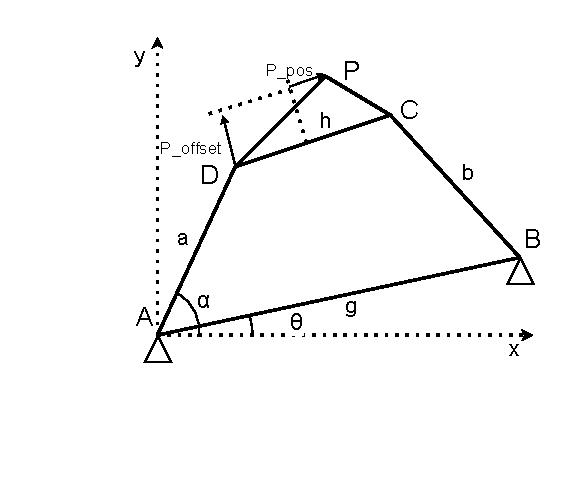
\includegraphics[width=0.5\textwidth]{./figures/four-bar_linkage+coupler_analysis.pdf}
	\end{center}
	\caption{Planar four-bar linkage with coupler $P$}
	\label{fig:four-bar_linakge_analysis}
\end{figure}
 
 After recalling all the input parameters we use them to find out the positions of the joints one by one.
 
 \begin{itemize}
 	\item Joint $A$.
 	
 	As previously mentioned, we position joint $A$ at $(0, 0)$ for simplicity. To place it at different coordinates, the whole linkage should be translated by adding the new coordinates of $A$ to each joint's coordinates.
 	
 	\item Joint $B$.
 	
 	The position of joint $B$ can be defined using $g$, the length of bar $AB$, and angle $\theta$: $B_x = g  \cos(\theta)$, $B_y = g \sin(\theta)$.
 	
 	\item Joint $D$.
 	
 	The position of joint $D$ is also easy to determine using $a$, the length of $AD$, and input angle $\alpha$: $D_x = a \cos(\alpha)$, $D_y = a \sin(\alpha)$.
 	
 	\item Joint $C$.
 	
 	The most complex problem is to determine the position of joint $C$. The main idea is to derive the position of $C$ by considering the area of triangle $\triangle BCD$ using different methods.
 	
 	To determine the position of $C$, we consider new basis vectors.
 	
 	Define a vector $\overrightarrow{BD} = (BD_x, BD_y) = \overrightarrow{D} - \overrightarrow{B} = (D_x - B_x, D_y - B_y)$. Assume first that this vector has non-zero length $|\overrightarrow{BD}| = \sqrt{(BD_x)^2+(BD_y)^2}$. 
 	
 	The corresponding unit vector along $\overrightarrow{BD}$ is $\overrightarrow{e}_{BD} = (e_{BD_-x}, e_{BD_-y}) = \frac{\overrightarrow{BD}}{|\overrightarrow{BD}|}$.
 	
 	The orthogonal direction is defined by a unit vector $\overrightarrow{n}_{BD} = (-e_{BD_-y}, e_{BD_-x})$.
 	
 	We use the vectors $\overrightarrow{e}_{BD}$ and $\overrightarrow{n}_{BD}$ as a new orthonormal basis.
 	
 	To determine the area of $\triangle BCD$ we use Heron's formula:
 	
 	$A_{\triangle BCD} = \sqrt{p (p-b) (p-h) (p-|\overrightarrow{BD}|)}$, where $p = \frac{b + h + |\overrightarrow{BD}|}{2}$ is a semi-perimeter of $\triangle BCD$.
 	
 	On the other hand the area of $\triangle BCD$ can be determined using length of $BD$ and the perpendicular from $C$ to $BD$ denoted by $C_{offset}$ (see Figure \ref{fig:four-bar_linakge_analysis}): $A_{\triangle BCD} = \frac{|\overrightarrow{BD}| C_{offset}}{2}$. So we can determine $C_{offset} = 2 \frac{A_{\triangle BCD}}{ |\overrightarrow{BD}|}$
 	
 	At this point, we know the distance from joint $C$ to $BD$ along $\overrightarrow{n}_{BD}$. To determine the position of $C$ with respect to $B$, we also need the distance from $C$ to $B$ along $\overrightarrow{e}_{BD}$. The projection length of $\overrightarrow{BC}$ onto direction of $\overrightarrow{e}_{BD}$ is given by $|C_{pos}| = \sqrt{b^2 - C_{offset}^2}$ using Pythagorean theorem. The remaining question is to determine sign of this projection. This can be done using angle $\angle CBD$ and the Law of Cosines: 
 	
 	$\cos(\angle CBD) = \frac{b^2 + |\overrightarrow{BD}|^2 - h^2}{2 b |\overrightarrow{BD}|}$
 	
 	Then the projection of $\overrightarrow{BC}$ onto direction of $\overrightarrow{e}_{BD}$ is given by $C_{pos} = sign(\cos(\angle CBD)) \sqrt{b^2 - C_{offset}^2}$
 	
 	After determining $C_{pos}$ and $C_{offset}$, we can find the possible positions of $C$:
 	
 	$\overrightarrow{C}_1 = (C_{1_-x}, C_{1_-y}) = \overrightarrow{B} + C_{pos} \overrightarrow{e}_{BD} + C_{offset} \overrightarrow{n}_{BD}$ 
 	
 	$\overrightarrow{C}_2 = (C_{2_-x}, C_{2_-y}) = \overrightarrow{B} + C_{pos} \overrightarrow{e}_{BD} - C_{offset} \overrightarrow{n}_{BD}$
 	
 	There are two possible positions of $C$, because the normal vector to $\overrightarrow{BD}$ is not unique and can also have the opposite direction. For a static structure, we can choose any of them, so we take $C = C_2$ as the default. For the animation case, that will be discussed later, there are rules for choosing between $C_1$ and $C_2$.
 	
 	In the discussion above we made the assumption that the length of $\overrightarrow{BD}$ is not zero. However, for $b = h$ and a specific value of input angle $\alpha$, the length can become zero. In this case, the joints $A$, $B$, $C$, $D$ are on the same line, so we define a unit vector $\overrightarrow{e} = sign(\overrightarrow{BA} \cdot \overrightarrow{BC})\frac{\overrightarrow{BA}}{g}$, where $\cdot$ is a scalar product. Then, the position of $C$ is determined uniquely by $\overrightarrow{C} = \overrightarrow{B} + b \overrightarrow{e}$
 	
 	\item Coupler $P$.
 	
 	Since we know the positions of $C$ and $D$, it is easy to determine the position of $P$.
 	
 	Define the midpoint of $CD$ as $\overrightarrow{Q} = \frac{\overrightarrow{C} + \overrightarrow{D}}{2}$.
 	
 	The unit vector along $DC$ is given by $\overrightarrow{e}_{DC} = (e_{DC_-x}, e_{DC_-y}) = \frac{\overrightarrow{C} - \overrightarrow{D}}{h}$. The corresponding normal vector is $\overrightarrow{n}_{DC} = (-e_{DC_-y}, e_{DC_-x})$.
 	
 	Then, the position of the coupler $P$ is determined by $\overrightarrow{P} = \overrightarrow{Q} + P_{pos} \overrightarrow{e}_{DC} + P_{offset} \overrightarrow{n}_{DC}$.
 	
 	Unlike the position of $C$, the position of $P$ is determined uniquely, because $P_{offset}$ can be specified as negative by the user, automatically changing the direction of $\overrightarrow{n}_{DC}$.
 \end{itemize}

 \subsection{Parameter Validation}
 
 Not every set of the input parameters is feasible. In this section we will derive constraints on the input angle $\alpha$ and the links' lengths to ensure that the linkage exists.
 
 \begin{figure}[h]
 	\centering
 	\begin{subfigure}{0.3\textwidth}
 		\centering
 		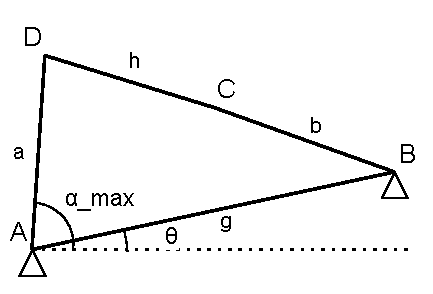
\includegraphics[width=\linewidth]{./figures/linkage_input_angle_limits_1.pdf}
 		\caption{Maximum input angle $\alpha$.}
 		\label{fig:max_alpha}
 	\end{subfigure}
 	\hfill
 	\begin{subfigure}{0.3\textwidth}
 		\centering
 		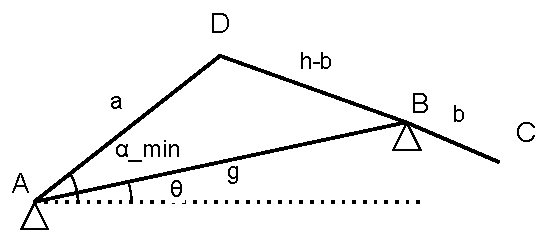
\includegraphics[width=\linewidth]{./figures/linkage_input_angle_limits_2.pdf}
 		\caption{Minimum input angle $\alpha$.}
 		\label{fig::min_alpha-1}
 	\end{subfigure}
 	\hfill
 	\begin{subfigure}{0.3\textwidth}
 	\centering
 	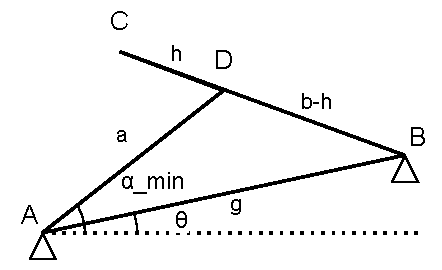
\includegraphics[width=\linewidth]{./figures/linkage_input_angle_limits_3.pdf}
 	\caption{Minimum input angle $\alpha$.}
 	\label{fig::min_alpha-2}
 	\end{subfigure}
 	\caption{Constraints on the input angle $\alpha$.}
 \end{figure}
 
 Figures \ref{fig:max_alpha}, \ref{fig::min_alpha-1}, \ref{fig::min_alpha-2} illustrate the cases of the maximum and minimum input angle $\alpha$. The coupler $P$ has no influence on the limits of the input angle therefore it is not shown in the figures. The limits of $\alpha$ are defined by the cases when the four-bar linkage folds into a triangle.
 
 \begin{itemize}
 \item Maximum input angle $\alpha$.
 
 Figure \ref{fig:max_alpha} displays the upper limit of the angle $\alpha$, that can be derived using the Law of Cosine for triangle $\triangle ABD$: $(h+b)^2 = a^2 + g^2 - 2 a g \cos(\alpha_{max}-\theta)$.
 
 If this cosine $\cos(\alpha_{max}-\theta) = \frac{a^2 + g^2 - (h+b)^2}{2 a g}$ has an absolute value less than one, there exists an upper limit for the input angle $\alpha$: $\alpha_{max} = \arccos(\frac{a^2 + g^2 - (h+b)^2}{2 a g}) + \theta$.
 
 \item Minimum input angle $\alpha$.
 
 Figures \ref{fig::min_alpha-1}, \ref{fig::min_alpha-2} show two different cases for minimum input angle $\alpha$. The both cases could be described using the Law of Cosine for triangle $\triangle ADB$: $(h-b)^2 = a^2 + g^2 - 2 a g \cos(\alpha_{min}-\theta)$.
 
 If this cosine $\cos(\alpha_{min}-\theta) = \frac{a^2 + g^2 - (h-b)^2}{2 a g}$ has an absolute value less than one, there exists a lower limit of the input angle $\alpha$: $\alpha_{min} = \arccos(\frac{a^2 + g^2 - (h-b)^2}{2 a g}) + \theta$.
 
 \item Special cases.
 
 If both cosines $\cos(\alpha_{min}-\theta)$ and $\cos(\alpha_{max}-\theta)$ have an absolute value greater or equal one, then there is no limits to the input angle $\alpha$.
 
 If only the maximum limit exists, then the input angle $\alpha$ also has a lower boundary, that is symmetric with respect to the ground link $AB$: $\alpha \in [\alpha_{max}, 2 \theta - \alpha_{max}]$.
 
 In the opposite case, when only the minimum input angle $\alpha$ exists, then the input angle is also bounded from above symmetrically with respect to the ground link $AB$: $\alpha \in [2 \theta + 2 \pi - \alpha_{min}, \alpha_{min}]$.
 \end{itemize}
 
 We decided that the GUI will display a slider for input angle $\alpha$, ensuring that only valid values within the boundaries can be entered by the user. A similar limitation can be derived for the output angle $\angle ABC$.
 
 There is also a case when the four-bar linkage does not exist for any input angle $\alpha$. This occurs when one of the bars is longer than the sum of other three, so that the quadrilateral $\square ABCD$ does not exist. Denote the longest bar as $l = \max(a, b, g, h)$, the shortest bar as $s = \min(a, b, g, h)$, and two remaining bars as $p$, $l$. Then the condition for linkage to exist is $l-p-q-s \le 0$. This condition will be checked by the four-bar linkage model, which will notify the user through the GUI in case of a problem.
 

 \subsection{Classification}
 
 After deriving the expressions for constraints on the input angle $\alpha$, we can classify the motion of four-bar linkage.
 
 Depending on the constraints on the input angle $\alpha$ and the output angle $\angle ABC$, the input link $AD$ and the output link $BC$ can be classified into four types according to \cite{inproceedings}.
 
 \begin{itemize}
 	\item \textit{Crank}.
 	
 	The link can rotate fully, with neither a minimum, nor a maximum for the input angle $\alpha$ (or the output angle $\angle ABC$).
 	
 	\item \textit{Rocker}.
 	
 	The link can rotate partially, with both a minimum and a maximum for the input angle $\alpha$ (or the output angle $\angle ABC$).
 	
 	\item \textit{0-rocker}.
 	
 	The link can rotate partially, with no minimum but with maximum for the input angle $\alpha$ (or the output angle $\angle ABC$).
 	
 	\item \textit{$\pi$-rocker}.
 	
 	The link can rotate partially, with no maximum but with minimum for the input angle $\alpha$ (or the output angle $\angle ABC$).
 \end{itemize}
 
 \subsection{27 Movement Cases}
 
 The classification of the input and output links implies, that there are different linkage types. For example, the input and output can independently be classified as cranks or rockers, leading to different linkage types. The study in \cite{inproceedings} identifies $27$ different combinations. These combinations can be described by signs of characteristic values: $T_1 = g + h - a - b$, $T_2 = b + g - h - a$ and $T_3 = b + h - g - a$. Since each characteristic value can be positive, negative, or zero, there are $27$ possible combinations and motion types respectively.
 
 Initially, we discussed to analyze the motion in each of $27$ cases separately. However, we decided to implement the general algorithms that handles all cases.
 

 \subsection{Animation}

 At the beginning of the animation, we start with a static state of the linkage. By default we set $C_2$ as the chosen position for joint $C$.
 The animation is implemented as a discrete process by gradually incrementing the input angle using the following key variables:
 \begin{itemize}
 	\item $dt$: Time interval of the animation.
 	\item $\dot{\alpha}$: constant angular velocity of the input angle $\alpha$.
 \end{itemize}

This is our basic idea of iterative animation:
\begin{itemize}
	\item Calculate the limit values of $\alpha$ described above.
	
	\item Update $\alpha$ using the following formula: $\alpha = \alpha \pm \dot{\alpha} dt$.
		 
	The sign here depends on the \texttt{direction} parameter. It determines whether $\alpha$ changes clockwise (\texttt{direction = 1}) or counterclockwise (\texttt{direction = 0}).
	 
	\item Use the updated $\alpha$ value to calculate other parameters, such as the positions of the joints.
		 
	\item If the input angle $\alpha$ is limited, then change the \texttt{direction} parameter at the limits to rotate the input link backwards.
		 
	\item If the input angle is not bounded, ensure that $\alpha$ always remains within the range $[0^\circ, 360^\circ]$. If the input angle exceeds $360^\circ$ or falls below $0^\circ$, we will reset it to the corresponding boundary value.
		 
	\item Switch between $C_1$ and $C_2$ to ensure continuity of animation.
	
	As we mentioned earlier, for the static configuration, we choose $C_2$ as the default position for joint $C$. However, during the motion, we need to switch between $C_1$ and $C_2$ to maintain continuous velocity due to the principle of inertia. This means that at every limit of the input angle we switch between $C_1$ and $C_2$.
	
	Note, that we need to switch even at the boundary cases, when the absolute values of $\cos(\alpha_{max}-\theta)$ or $\cos(\alpha_{min}-\theta)$ are equal to one, indicating that the input angle has reached its extreme positions.

	\item Consider floating point precision.
	
	To avoid issues caused by floating point inaccuracies when checking if the cosine value of $\alpha$ approaches $-1$ or $1$, we incorporate floating point tolerance of $10^{-10}$.
\end{itemize}


\section{Design} \label{ch:design}

After completing the analysis part we begin to design the software that will be implemented later. Our design section consists of two parts, the selection of development infrastructure and the creation of class diagrams to be a basis for implementation.

\subsection{Third-Party Software and Development Infrastructure}

Since we now understand the problem that we need to solve, we can choose an implementation environment.

We decided to implement our project using Python. This decision is based on several key factors:
\begin{itemize}
	\item Python has a numpy\footnote{\label{fn:numpy} https://numpy.org/} library that deals well with vector operations. The four-bar linkage model requires solving geometrical problem, so the built-in vector and matrix operations are highly desired to simplify the code.
	\item Python has a standard GUI library tkinter\footnote{\label{fn:tkinter} https://docs.python.org/3/library/tkinter.html}.
	\item Most of the team members have more experience with Python than with C++.
\end{itemize}

There is a list of the software and tools we used for implementation:
\begin{itemize}
	\item Operating systems: Xubuntu and Windows.
	\item Programming language: Python.
	\item Integrated development environment (IDE): Spyder\footnote{https://www.spyder-ide.org/} and PyCharm\footnote{https://www.jetbrains.com/pycharm/}.
	\item Package manager: Anaconda\footnote{https://www.anaconda.com/}.
	\item Libraries: tkinter\textsuperscript{\ref{fn:tkinter}}, numpy\textsuperscript{\ref{fn:numpy}}, math\footnote{https://docs.python.org/3/library/math.html}, unittest\footnote{https://docs.python.org/3/library/unittest.html}.
	\item Version control system: GitHub repository\footnote{\url{https://github.com/einsflash/Project_Pusher_Mechanism}}.
	\item Documentation: Pdoc\footnote{https://pdoc.dev/docs/pdoc.html}
\end{itemize}

\subsection{Class Models}

In the project we need to store a large amount of variables for geometric representation and visualization of the four-bar linkage, as well as for corresponding tools like buttons und sliders. The number of variables is too large to pass it into different functions as arguments. Therefore, we decided to implement the four-bar linkage model and the GUI as two separate classes, so every member function will have an access to the data stored in the class without passing it as an argument.

\begin{figure}[h]
	\begin{center}
		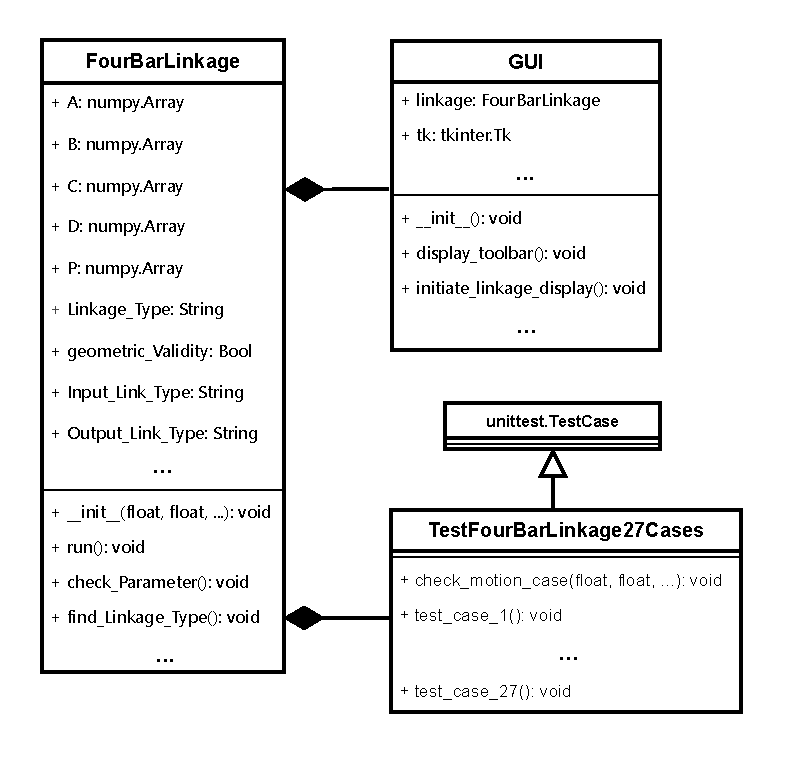
\includegraphics[width=0.65\textwidth]{./figures/class_diagram.pdf}
	\end{center}
	\caption{UML class diagram}
	\label{fig:class diagram}
\end{figure}

Figure \ref{fig:class diagram} shows a shortened version of the class diagram. This diagram illustrates all the relationships between classes and the most important attributes. The actual number of attributes is too high to include it in this document, the comprehensive class diagram can be found in our GitHub repository\footnote{\url{https://github.com/einsflash/Project_Pusher_Mechanism/blob/main/src/class_diagram.pdf}}.

The backend class \texttt{FourBarLinkage} implements the geometry and animation of the four-bar linkage with a coupler. The number of member variables is large, but the most important for visualization are the coordinates of joints $A$, $B$, $C$, $D$, and $P$. There are also member variables used for classification (\texttt{Linkage\_Type}, \texttt{Input\_Link\_Type}, \texttt{Output\_Link\_Type}) and for input validation (\texttt{geometric\_Validity}) to notify GUI about invalid parameters. The main member functions are the constructor \texttt{\_\_init\_\_} to set geometrical parameters, \texttt{run} to compute the joints' coordinates, \texttt{check\_Parameter} to validate user input, and \texttt{find\_Linkage\_Type} to classify the linkage. There are many other attributes used for internal purposes, but they are less important for a general overview.

The frontend class \texttt{GUI} is used to create the graphical user interface to visualize linkage, provide its animation and get geometrical parameters from the user. This class has also a large number of attributes, but only several of them are important for an overview. The member variables include an instance of the \texttt{FourBarLinkage} class, which is used to obtain joint coordinates for visualization and animation. The \texttt{GUI} class also contains an instance of \texttt{tkinter.Tk}, the basic class for creating GUI using tkinter. The main member functions are the constructor \texttt{\_\_init\_\_} to initiate the GUI, \texttt{display\_toolbar} to set up the toolbar of buttons, sliders, and other elements, and \texttt{initiate\_linkage\_display} to set up the visualization of the linkage.

The test class \texttt{TestFourBarLinkage27Cases} inherits from \texttt{unittest.TestCase} and is used to test all motion types of the linkage. This class has only member functions that implement test cases for each motion types.

\section{Implementation} \label{ch:implementation}

\subsection{Backend}
e.g. validation of input parameters

\subsection{Frontend}

overview of source code structure (file names, directories); build instructions; references into source code documentation e.g, doxygen\footnote{\tt https://github.com/doxygen/doxygen}; short (!) code listings
\begin{lstlisting}
#include<iostream>
int main() {
  std::cout << "Leave me alone world!" << std::endl;
  return 42;
}
\end{lstlisting}
if helpful (must come with detailed explanation)

\subsection{Software Tests}

e.g, googletest\footnote{\tt https://github.com/google/googletest}

\section{Documentation}\label{ch:doc}

\section{Optimization Problem}\label{ch:optimization-problem}


\section{Project Management} \label{ch:projectmanagement}

who did what, when, and why; organization of collaboration, i.e. [online] meetings, software version control (e.g, git\footnote{\tt https://git.rwth-aachen.de}

\bibliographystyle{plain}
\bibliography{literature}

\appendix

\section{User Documentation} \label{ch:userdoc}

\subsection{Building}

e.g, using cmake\footnote{\tt https://cmake.org/} and make\footnote{\tt https://www.gnu.org/software/make/}


\subsection{Testing}

e.g, \verb!make test!

\subsection{Running}

documented sample session(s); e.g, \verb!make run!


\end{document}

